\documentclass{article}
%\documentclass{report} % Can be article, report, book, anything you want!

\usepackage{vub} % this will automatically set to A4 paper. We're not in the US.
% if, for some obscure reason, you need another format, please file an issue (see further).

% The `vub` package has many options.
% Please read the documentation at https://gitlab.com/rubdos/texlive-vub if you want to learn about them.

% Feel free to mix and match with other packages.
\setlength{\parskip}{10pt}  % Adjust the space between paragraphs
\usepackage{hyperref}
\usepackage{float}
\usepackage{tabularx}
\usepackage{graphicx}
\graphicspath{{../src/report/images/}{./images/}}

\title{Key-Value Store}
\subtitle{Multicore Programming: Project Erlang}
\faculty{Sciences and Bio-Engineering Sciences} % Note: without the word "Faculty"!
\author{Gérard Lichtert \\
\href{mailto:gerard.lichtert@vub.be}{gerard.lichtert@vub.be}}

\begin{document}
\maketitle

\tableofcontents
\newpage
\raggedright

\section{Overview}
To give a brief summary of the reports' contents, we will first start with the
implementation, which discusses a sharded and cached implementation (henceforth
called the 'sharded' implementation). The sharded implementation distributes
each store in an actor (called bucket) and keeps a central actor to coordinate communication
between clients and the buckets. Another implementation that is discussed is a
worker, sharded and cached implementation (henceforth called the 'worker'
implementation). This implementation is similar to the previous in regards of
the buckets, however whenever a client connects to the server, they get their
own process to communicate with. So this implementation has a one to one process
relation whilst the previous has many to one relation.
\par
These implementations together with the provided central implementation are used
to perform some experiments. The first experiment measures the speedup,
depending on the number of scheduler threads. The second measures throughput
depending on the number of scheduler threads. Both of these experiments use the
worker implementation to analyze the results, however the results for the other
implementations are also available in the dataset.
The last compares the throughput of the different implementations
\section{Implementation}
\subsection{Central implementation}
\subsubsection{Architecture}
To start explaining the implementations, we will start out with the provided
central implementation, which is just a single process containing a dictionary
of dictionary, or a dictionary of buckets, to which the user sends CRUD (Create,
Read, Update, Delete) messages. The single process or 'Server' handles all the
messages and also responds to them after performing the necessary operations. A
diagram showcasing the flow of the messages can be seen in
\autoref{fig:central-implementation}.
\begin{figure}[h!]
	\centering
	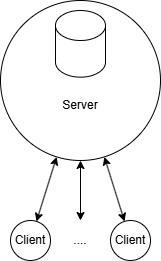
\includegraphics[width=0.2\textwidth]{central.png}
	\caption{Message flow of the Central implementation}
	\label{fig:central-implementation}
\end{figure}
As this implementation was meant to be improved upon for scalability, we will not be
answering the scalability questions for this implementation.
\newpage
\subsection{Sharded-Cached implementation}
\subsubsection{Architecture}
To split the central implementation up, instead of having a nested dictionary,
we create a process per bucket, so each bucket process will hold a
dictionary or the Key-Value store and the central process will keep track of the process ID's in its
dictionary to address each bucket. This means that while the central process still has to handle all
communication from the clients, it no longer has to manage the data by itself
only the addresses of the buckets.
The only responsability that the server has is to create the buckets when needed
and forward the messages of the client to the appropiate bucket. The
responsability of the buckets is to perform the operations that the server
forwards to it and to respond to the clients. A diagram showing the flow of
communication can be seen in \autoref{fig:sharded-implementation}.\\
\begin{figure}[h]
	\centering
	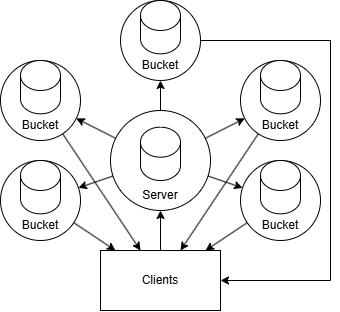
\includegraphics[width=0.3\textwidth]{sharded-implementation.png}
	\caption{Message flow of the Sharded implementation}
	\label{fig:sharded-implementation}
\end{figure}
To improve on the performance of the implementation we also add a caching
mechanism that remembers the last bucket addressed in the server. If a message
is to be forwarded to the same bucket twice or more in a row, the server no
longer needs to look the bucket up since it already has the address.
This mechanism is also applied in the buckets for retrieval operations, where it
remembers the last value associated with the last lookup.
\subsubsection{Scalability}
This implementation allows the system to scale with the amount of key-value
stores that exist, since each gets its own process to live in, and the load gets
split to the buckets themselves. The best case would be if the clients operate
on different buckets and the worst case would be if all clients operate on the
same bucket. However since the bottleneck is the server, the load on the buckets
will at most be the same as the server.
\subsection{Worker-Sharded-Cached implementation}
To improve on the Sharded implementation, we need to solve the bottleneck in the
server. Currenty all communication of all the clients go through the server and
get forwarded to the appropiate buckets which is cumbersome for the server. To
aleviate the server we create a worker process for each client that connects to
the server, and in doing so, each client will have its own worker to which it
sends messages to. \\
The worker will in turn forward the messages to the appropiate bucket. The only
issue with this implementation is that when a client creates a bucket, the
bucket must also be available to all the other clients connected to the service.
To solve this we add the responsability of replicating the address of the bucket
to the server. The server keeps track of all existing worker processes and
whenever one of them send a replication message (when a new bucket is created),
it broadcasts it to the rest of the existing worker processes, which add the
bucket to their dictionary of buckets. An example of this is shown in the
diagram in \autoref{fig:worker-bucket-creation-process}.\par
\begin{figure}[H]
	\centering
	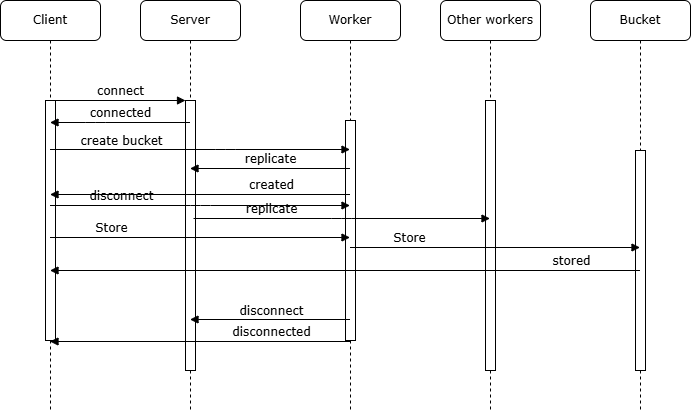
\includegraphics[width=0.7\textwidth]{worker-bucket-creation-process.png}
	\caption{Creating a bucket in the Worker implementation}
	\label{fig:worker-bucket-creation-process}
\end{figure}
To keep making use of the caching mechanism, it is moved from the server to the
worker process, since the workers keep track of the buckets that the client
interacts with. Moreover, since it will always be the same client interacting
with the worker, the cache will be hit more frequently. \\
A general flow of messages can be seen in \autoref{fig:worker-implementation}.
\begin{figure}[H]
	\centering
	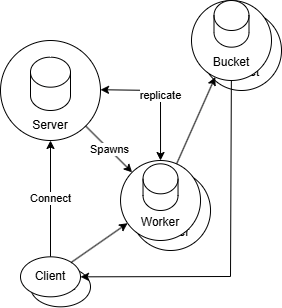
\includegraphics[width=0.4\textwidth]{worker-implementation.png}
	\caption{Message flow of the Worker implementation}
	\label{fig:worker-implementation}
\end{figure}
\subsection{Scalability}
This implementation is a lot more scalable than the previous implementation. It
now allows the system to also scale with the amount of clients and thus allows
for messages to be processed in parallel. The best case would be if the client
on different buckets, allowing the load to be distributed across the buckets.
The worst case would be if all the clients operate on a single bucket, creating
a bottleneck in the bucket. Since this implementation allows for the
parallelisation of the sent messages, the bottleneck there is now the speed of
the processing of the messages. Another bottleneck would be the buckets
themselves, if they receive more messages than they can handle. For this we
could explore further sharding of the bucket, or replication as well as pla:!cing
the bucket behind a load balancer.
\newpage
\section{Evaluation}
\subsection{Experimental set-up}
\label{sec:experimental-set-up}
For the experiments I used two devices. Firstly the Firefly machine of the VUB
and my own laptop henceforth called "Omen" to set up the experiments for Firefly
as well as make the necessary scripts and programs to run the experiments on
firfly and analyze the data automatically. The specifications of both devices
are found in \autoref{table:hardware}
\begin{table}[H]
	\centering
	\begin{tabularx}{\textwidth}{c | X | X}
		Device                       & Firefly                                                   & Omen HP laptop            \\
		\hline
		\textbf{Hardware}            &                                                           &                           \\
		CPU                          & AMD Ryzen Threadripper 3990X Processor
		(64 cores / 128 threads @
		2.9 GHz Base, 4.3 GHz boost) & Intel Core i7-9750H (6 cores / 12 threads) @ 2.6 GHz, 4.5
		Ghz boost                                                                                                            \\
		\hline
		RAM                          & 128 GB (DDR4 3200 MHz)
		                             & 16GB (DDR4 2667 MHz)                                                                  \\
		\hline
		\textbf{Software}            &                                                           &                           \\
		OS                           & Ubuntu 24.04.1                                            & Microsoft Windows 11 Home \\
		\hline
		Erlang/OTP version           & 25.3.2.8                                                  & 27                        \\
	\end{tabularx}
	\caption{Hardware used for the experiments}
	\label{table:hardware}
\end{table}
For the experiments I used a Powershell script and a Bash script to start an
erlang process to perform an experiment and benchmark it 30 times. This was done
for each implementation, so for the central, sharded and worker implementation
and for three different scenarios. The scenarios were: A read only scenario,
where clients only send retrieve messages to the server. A read write scenario
where clients performed 50-50 writes and reads. Finally also a mixed scenario
where the balance was 90\% reads and 10\% writes. Note that only the time
elapsed for performing these operations was measured and thus the buckets were
already existing prior to starting the benchmark. \par
Each experiment has 100 clients performing operations on the system. Each client
will do 1000 operations per scenario and 2000 operations in the read-write
scenario. There will always be 1000 buckets, each holding 100 keys.
\subsection{Experimental methodology}
To measure the time elapsed we used the wall clock time on the client side and we performed the
experiment 64 times per scenario and per implementation on the Omen device, once
per amount of scheduler threads (so 1-64). On Firefly we performed the
experiment 128 times per scenario, per implementation since it can use a lot
more threads.
\subsection{Experiments}
For the first experiment we will be comparing the throughput of the different
implementations on the maximum amount of scheduler threads (12 for Omen and 128
for Firefly).
\subsubsection{Throughput per second depending on the implementation and
	scenario}
For this experiment we use the parameters mentioned in
\autoref{sec:experimental-set-up}. For each device we use the measurements for
the maximum amount of threads, so in Omen's case its 12 and for Firefly its 128.
\begin{figure}[H]
	\centering
	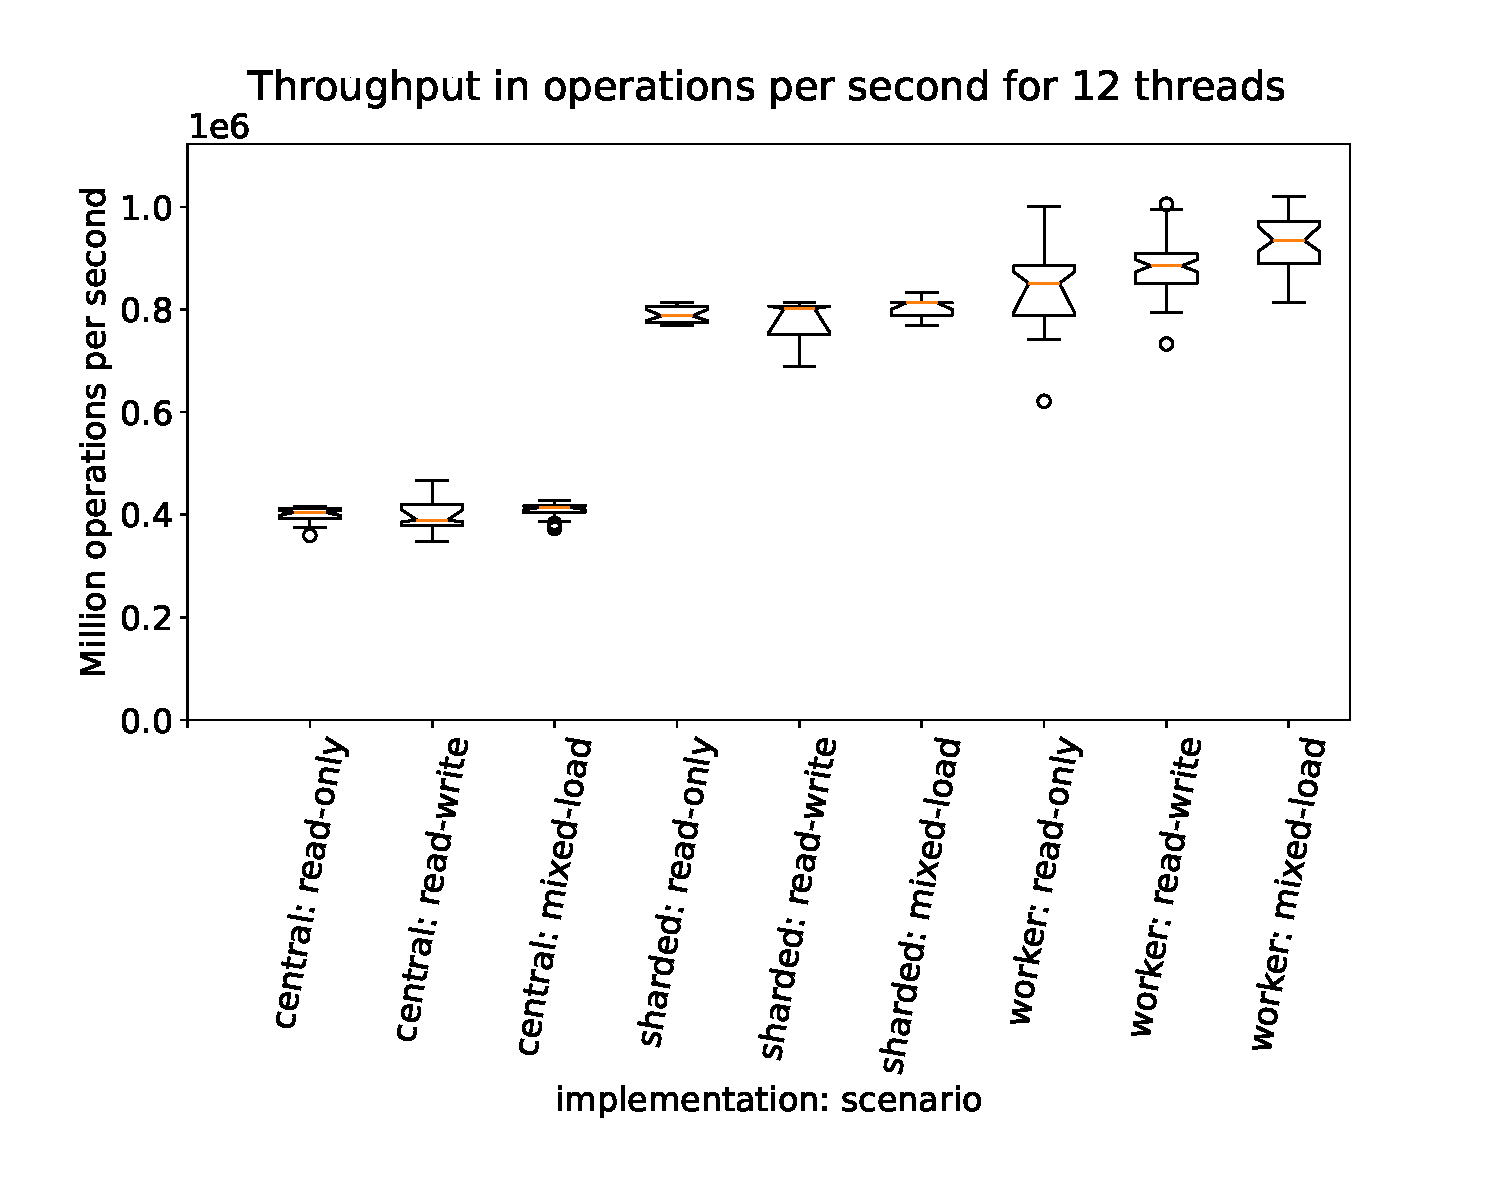
\includegraphics[width=0.8\textwidth]{boxplots/omen/boxplot-throughput-in-operations-per-second-for-12-threads.pdf}
	\caption{Comparing throughput of implementations on Omen}
	\label{fig:throughput-compare-impl-omen}
\end{figure}
On Omen we can clearly see an improving trend in terms of the throughput when
improving the implementations, however the returns seem to be diminishing. The
difference between the central implementation and the sharded implementation is
clear. The sharded implementation is a clear imrovement. Comparing the sharded
and the worker implementation might require you to squint your eyes a little as
the there is not always an improvement. Most of the the time there is an
improvement but in some cases outliers perform worse than the sharded
implementation. In the case of read only operations the throughput even overlaps
with the sharded implementation.

% On firefly

\subsection{Throughput per second depending on scheduler threads}
\label{sec:throughput-per-second-depending-on-scheduler-threads}
For this experiment we use the same parameters mentioned in
\autoref{sec:experimental-set-up} but set the scenario to read-write, as it
provides the results of a balanced mix of operations and requires more
operations to complete. We will also only look at the worker implementation as
it seems to have the most potential for the highest throughput. In this experiment we measure the throughput of
operations depending on the amount of scheduler threads. For Omen, we will look
at 1-12 threads and for firefly 1-128.
\begin{figure}[H]
	\centering
	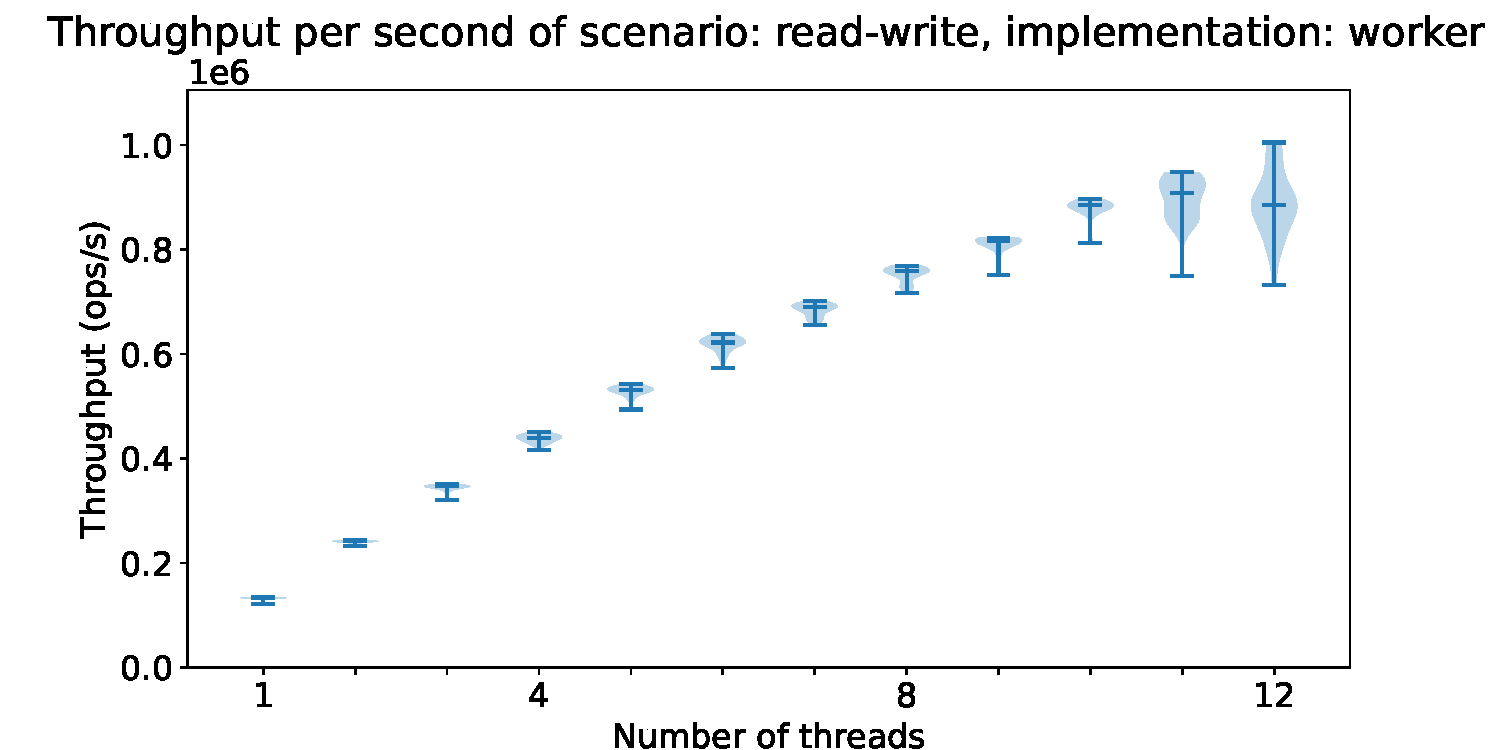
\includegraphics[width=0.8\textwidth]{violinplots/omen/throughput-per-second-of-scenario-read-write-implementation-worker-violinplot.pdf}
	\caption{Throughput Omen, impl: worker, scenario: read-write}
	\label{fig:throughput-omen-read-write-depend-threads}
\end{figure}
Looking at the results from Omen, we can see that there is a general trend that
improves the throughput as we add more threads. However the returns are
diminishing as the curve is logarithmic. In the last two measurements (11 and 12
threads) we can see that they are very similar. While having 12 threads makes it
possible to outperform 11 threads, it is not implied as some results seem to
overlap or are worse.
\subsection{Speedup depending on scheduler threads}
For this experiment we will use the same parameters mentioned in
\autoref{sec:experimental-set-up} and similar variables as in
\autoref{sec:throughput-per-second-depending-on-scheduler-threads}. We will only
be looking at the worker implementation and at the read-write scenario.
Furthermore, we will use the median of the results of the single threaded
experiment as the basis to compute the speedup for multiple threads.
\begin{figure}[H]
	\centering
	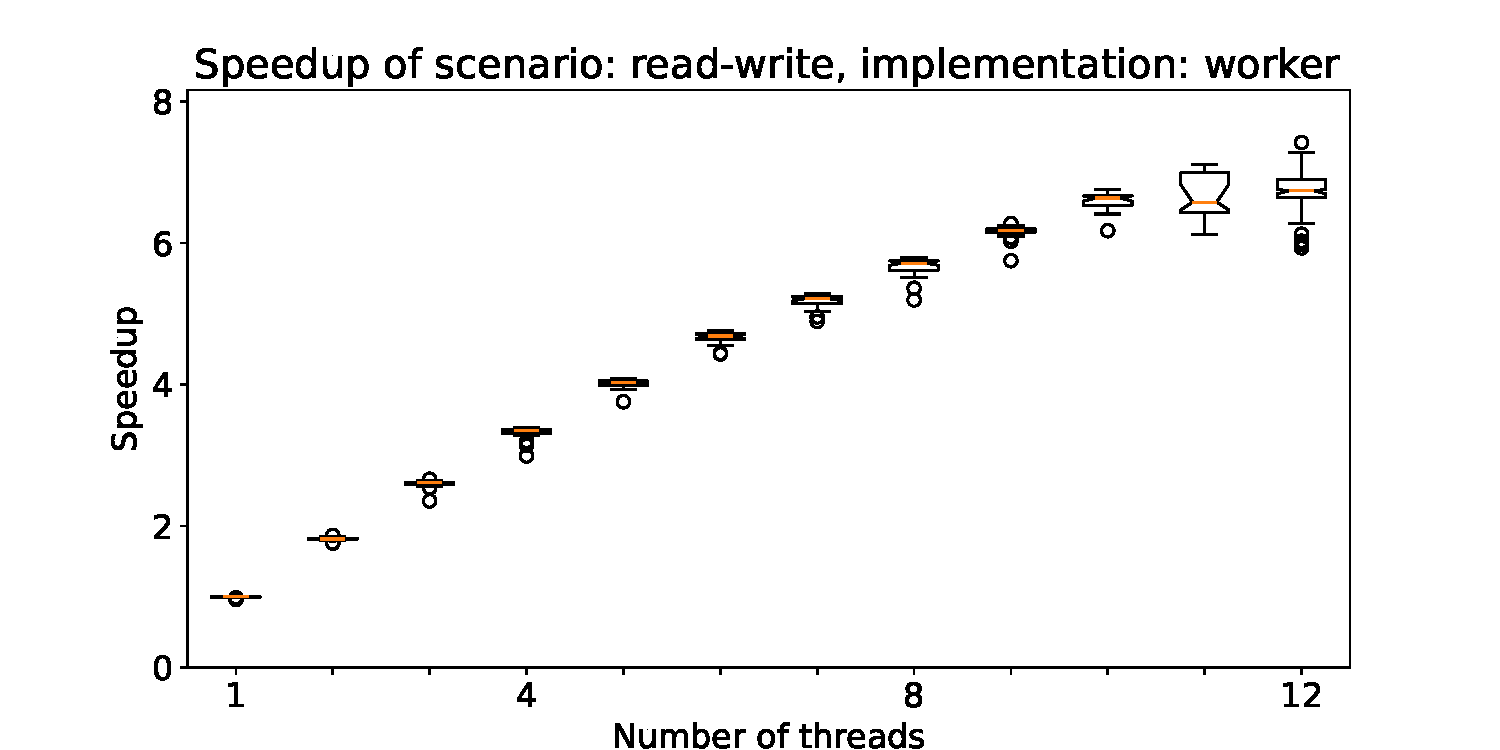
\includegraphics[width=0.8\textwidth]{boxplots/omen/boxplot-speedup-of-scenario-read-write-implementation-worker.pdf}
	\caption{Speedup on Omen, impl: worker, scenario: read-write}
	\label{fig:speedup-omen-worker-rw}
\end{figure}
Similar to the previous experiment, we can see in \autoref{fig:speedup-omen-worker-rw} that there is an improving trend, however once
12 threads are used the results seem to have the potential to be better than 11
threads but are not always better.
Comparing the difference in medians between threads: $$\Delta Speedup(T) =
	Median(Speedup(T)) - Median(Speedup(T - 1))\:with\:T=\#Threads$$
\begin{figure}[H]
	\centering
	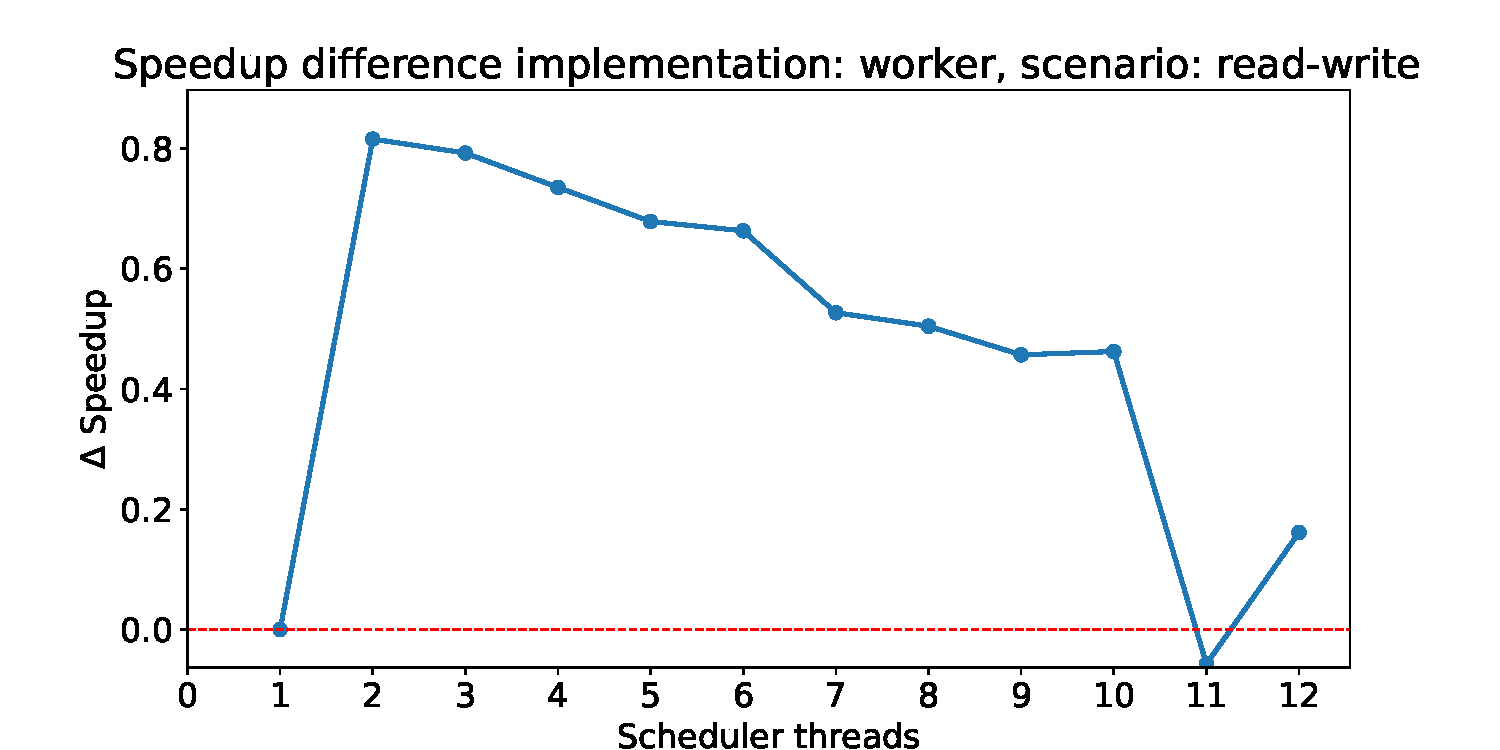
\includegraphics[width=0.8\textwidth]{plot/omen/plot-speedup-difference-implementation-worker-scenario-read-write.pdf}
	\caption{$\Delta Speedup$ Omen read-write}
	\label{fig:delta-speedup-omen-rw}
\end{figure}
in \autoref{fig:delta-speedup-omen-rw} we can clearly see the downwards trend of
improvements when adding an extra thread.
\section{Insight}
\subsection{Lightweight processes and its impact}
The lightweight-ness of the processes has definately influenced my solution,
because in other languages they have a hefty additional cost to create. This
means that there is usually an optimal amount of processes you can have before
your speedup starts to actually decrease. In Erlang however, the
worker implementation can scale to 100 users and 100 buckets, having 201
processes in total without any issues and still packs a punch. Consequently
I don't restrain myself as much as in the other languages in terms of the amount of processes created.
If the processes did cost much higher, I would probably be looking for an
optimal amount of processes to have to reach the optimal performance and base my
implementation on that instead of going nuts with the amount of processes.
\subsection{Distribution of cores over multiple machines}
If the application would be distributed over multiple machines, the achitecture
or the worker implementation would still be viable, but on a larger scale. This
means that perhaps it would be better to give each process or each X amount of
processes a machine. Since my implementation now primarily focusses on
processing the most amount of requests in the least amount of time, I would
probably shift my focus to avoiding network requests since these are responsible
for most of the
latency in operations. I would probaby be looking to keep a cache of the Bucket
as close to the user as possible, Maybe even the bucket and the worker process
as close together as possible, so I would probably be looking at minimizing physical
distances as well. Some other techniques might be to replicate the buckets and have a
load balancer in front of them. \par
To distribute processes to different machines, I would write a script that
activates the Erlang shell with the right parameters. This allows your local
computer to spawn processes on the remote computer with an Erlang program, which
is run after activating the Erlang shell on the remote machine.
\end{document}
